\chapter{计算几何}

\index{geometry}

在几何问题中，困难往往在于找到一种既便于实现、特殊情况又尽可能少的解题方法。

例如，给定一个四边形（具有四个顶点的多边形）的各个顶点，要求计算其面积。一种可能的输入如下：

\begin{center}
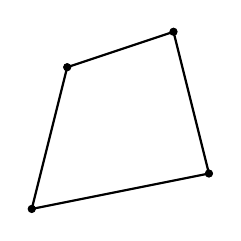
\begin{tikzpicture}[scale=0.45]

\draw[fill] (6,2) circle [radius=0.1];
\draw[fill] (5,6) circle [radius=0.1];
\draw[fill] (2,5) circle [radius=0.1];
\draw[fill] (1,1) circle [radius=0.1];
\draw[thick] (6,2) -- (5,6) -- (2,5) -- (1,1) -- (6,2);
\end{tikzpicture}
\end{center}
一种方法是连接两个相对顶点，用直线把四边形分成两个三角形：
\begin{center}
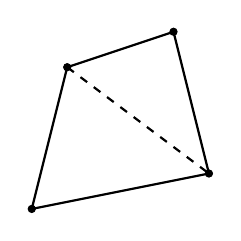
\begin{tikzpicture}[scale=0.45]

\draw[fill] (6,2) circle [radius=0.1];
\draw[fill] (5,6) circle [radius=0.1];
\draw[fill] (2,5) circle [radius=0.1];
\draw[fill] (1,1) circle [radius=0.1];

\draw[thick] (6,2) -- (5,6) -- (2,5) -- (1,1) -- (6,2);
\draw[dashed,thick] (2,5) -- (6,2);
\end{tikzpicture}
\end{center}
随后只需把两个三角形的面积相加。三角形面积可用\key{海伦公式}计算：
%\footnote{Heron of Alexandria (c. 10--70) was a Greek mathematician.}
\[ \sqrt{s (s-a) (s-b) (s-c)},\]
其中 $a$、$b$、$c$ 是三角形三边长度，$s=(a+b+c)/2$。
\index{Heron's formula}

这种解法可行，但存在一个陷阱：应如何把四边形分成三角形？事实证明，有时不能任意选取一对相对顶点。例如，在下图中，分割线位于四边形\emph{外部}：
\begin{center}
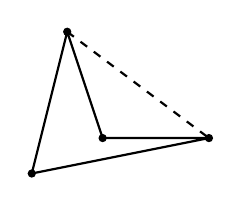
\begin{tikzpicture}[scale=0.45]

\draw[fill] (6,2) circle [radius=0.1];
\draw[fill] (3,2) circle [radius=0.1];
\draw[fill] (2,5) circle [radius=0.1];
\draw[fill] (1,1) circle [radius=0.1];
\draw[thick] (6,2) -- (3,2) -- (2,5) -- (1,1) -- (6,2);

\draw[dashed,thick] (2,5) -- (6,2);
\end{tikzpicture}
\end{center}
不过，换一条分割线就可以：
\begin{center}
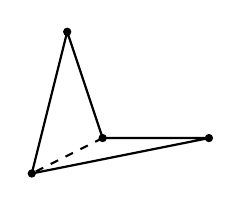
\begin{tikzpicture}[scale=0.45]

\draw[fill] (6,2) circle [radius=0.1];
\draw[fill] (3,2) circle [radius=0.1];
\draw[fill] (2,5) circle [radius=0.1];
\draw[fill] (1,1) circle [radius=0.1];
\draw[thick] (6,2) -- (3,2) -- (2,5) -- (1,1) -- (6,2);

\draw[dashed,thick] (3,2) -- (1,1);
\end{tikzpicture}
\end{center}
人很容易判断哪条分割线正确，但计算机处理起来并不容易。

不过，可以改用一种更便于编程的方法。存在如下通用公式：
\[x_1y_2-x_2y_1+x_2y_3-x_3y_2+x_3y_4-x_4y_3+x_4y_1-x_1y_4,\]
它可以计算顶点为
$(x_1,y_1)$,
$(x_2,y_2)$,
$(x_3,y_3)$ and
$(x_4,y_4)$ 的四边形面积。该公式易于实现，没有特殊情况，而且还能推广到\emph{所有}多边形。

\section{复数}

\index{complex number}
\index{point}
\index{vector}

\key{复数}形如 $x+y i$，其中 $i = \sqrt{-1}$ 是\key{虚数单位}。复数的几何意义是表示二维点 $(x,y)$，或从原点指向 $(x,y)$ 的向量。

例如，$4+2i$ 对应下面的点和向量：

\begin{center}
\begin{tikzpicture}[scale=0.45]

\draw[->,thick] (-5,0)--(5,0);
\draw[->,thick] (0,-5)--(0,5);

\draw[fill] (4,2) circle [radius=0.1];
\draw[->,thick] (0,0)--(4-0.1,2-0.1);

\node at (4,2.8) {$(4,2)$};
\end{tikzpicture}
\end{center}

\index{complex@\texttt{complex}}

C++ 的复数类 \texttt{complex} 在解决几何问题时十分有用。它可以用复数表示点和向量，并提供多种适用于几何计算的工具。

在下面的代码中，\texttt{C} 是坐标类型，\texttt{P} 是点或向量的类型。代码还定义了宏 \texttt{X} 和 \texttt{Y}，用于访问 x、y 坐标。

\begin{lstlisting}
typedef long long C;
typedef complex<C> P;
#define X real()
#define Y imag()
\end{lstlisting}

例如，下面的代码定义点 $p=(4,2)$，并输出其 x、y 坐标：

\begin{lstlisting}
P p = {4,2};
cout << p.X << " " << p.Y << "\n"; // 4 2
\end{lstlisting}

下面的代码定义向量 $v=(3,1)$ 和 $u=(2,2)$，再计算它们的和 $s=v+u$。

\begin{lstlisting}
P v = {3,1};
P u = {2,2};
P s = v+u;
cout << s.X << " " << s.Y << "\n"; // 5 3
\end{lstlisting}

实践中，坐标通常适合用 \texttt{long long}（整数）或 \texttt{long double}（实数）表示。应尽可能使用整数，因为整数计算是精确的。若必须使用实数，比较数值时要考虑精度误差。判断实数 $a$ 与 $b$ 是否相等的一种安全方法是检查 $|a-b|<\epsilon$，其中 $\epsilon$ 是很小的数（例如 $\epsilon=10^{-9}$）。

\subsubsection*{函数}

以下示例中的坐标类型为 \texttt{long double}。

函数 $\texttt{abs}(v)$ 用公式 $\sqrt{x^2+y^2}$ 计算向量 $v=(x,y)$ 的长度 $|v|$。它也可用于计算点 $(x_1,y_1)$ 与 $(x_2,y_2)$ 之间的距离，因为该距离等于向量 $(x_2-x_1,y_2-y_1)$ 的长度。

下面的代码计算点 $(4,2)$ 与 $(3,-1)$ 之间的距离：
\begin{lstlisting}
P a = {4,2};
P b = {3,-1};
cout << abs(b-a) << "\n"; // 3.16228
\end{lstlisting}

函数 $\texttt{arg}(v)$ 计算向量 $v=(x,y)$ 相对于 x 轴的夹角。返回值以弧度表示，$r$ 弧度等于 $180 r/\pi$ 度。指向右方的向量角度为 0；顺时针旋转时角度减小，逆时针旋转时角度增大。

函数 $\texttt{polar}(s,a)$ 构造长度为 $s$、方向角为 $a$ 的向量。向量乘以一个长度为 1、方向角为 $a$ 的向量，即可将其旋转 $a$ 弧度。

下面的代码先计算向量 $(4,2)$ 的方向角，再将它逆时针旋转 $1/2$ 弧度，最后重新计算方向角：

\begin{lstlisting}
P v = {4,2};
cout << arg(v) << "\n"; // 0.463648
v *= polar(1.0,0.5);
cout << arg(v) << "\n"; // 0.963648
\end{lstlisting}

\section{点与直线}

\index{cross product}

向量 $a=(x_1,y_1)$ 与 $b=(x_2,y_2)$ 的\key{叉积} $a \times b$ 为 $x_1 y_2 - x_2 y_1$。把 $b$ 接在 $a$ 之后时，叉积可以判断 $b$ 是向左转（正值）、不转向（零）还是向右转（负值）。

下图展示了这三种情况：
\begin{center}
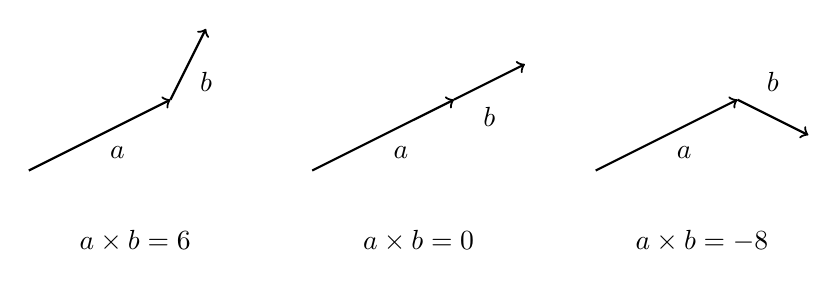
\begin{tikzpicture}[scale=0.45]

\draw[->,thick] (0,0)--(4,2);
\draw[->,thick] (4,2)--(4+1,2+2);

\node at (2.5,0.5) {$a$};
\node at (5,2.5) {$b$};

\node at (3,-2) {$a \times b = 6$};

\draw[->,thick] (8+0,0)--(8+4,2);
\draw[->,thick] (8+4,2)--(8+4+2,2+1);

\node at (8+2.5,0.5) {$a$};
\node at (8+5,1.5) {$b$};

\node at (8+3,-2) {$a \times b = 0$};

\draw[->,thick] (16+0,0)--(16+4,2);
\draw[->,thick] (16+4,2)--(16+4+2,2-1);

\node at (16+2.5,0.5) {$a$};
\node at (16+5,2.5) {$b$};

\node at (16+3,-2) {$a \times b = -8$};
\end{tikzpicture}
\end{center}

\noindent
例如，在第一种情况中 $a=(4,2)$、$b=(1,2)$。下面用 \texttt{complex} 类计算叉积：

\begin{lstlisting}
P a = {4,2};
P b = {1,2};
C p = (conj(a)*b).Y; // 6
\end{lstlisting}

上述代码之所以成立，是因为函数 \texttt{conj} 会把向量的 y 坐标取反；将向量 $(x_1,-y_1)$ 与 $(x_2,y_2)$ 相乘后，结果的 y 坐标正是 $x_1 y_2 - x_2 y_1$。

\subsubsection{点的位置}

叉积可用于判断一个点位于直线的左侧还是右侧。假设直线经过 $s_1$、$s_2$，观察方向从 $s_1$ 指向 $s_2$，待判断的点为 $p$。

例如，下图中的 $p$ 位于直线左侧：
\begin{center}
\begin{tikzpicture}[scale=0.45]
\draw[dashed,thick,->] (0,-3)--(12,6);
\draw[fill] (4,0) circle [radius=0.1];
\draw[fill] (8,3) circle [radius=0.1];
\draw[fill] (5,3) circle [radius=0.1];
\node at (4,-1) {$s_1$};
\node at (8,2) {$s_2$};
\node at (5,4) {$p$};
\end{tikzpicture}
\end{center}

叉积 $(p-s_1) \times (p-s_2)$ 可以判断点 $p$ 的位置。若叉积为正，$p$ 位于左侧；若为负，$p$ 位于右侧；若为零，则 $s_1$、$s_2$、$p$ 三点共线。

\subsubsection{线段相交}

\index{line segment intersection}

下面考虑如何判断两条线段 $ab$ 与 $cd$ 是否相交。可能情况如下。

\textit{情况 1：}
两条线段位于同一直线上，并且彼此重叠。此时有无穷多个交点。例如，在下图中，$c$ 与 $b$ 之间的所有点都是交点：
\begin{center}
\begin{tikzpicture}[scale=0.9]
\draw (1.5,1.5)--(6,3);
\draw (0,1)--(4.5,2.5);
\draw[fill] (0,1) circle [radius=0.05];
\node at (0,0.5) {$a$};
\draw[fill] (1.5,1.5) circle [radius=0.05];
\node at (6,2.5) {$d$};
\draw[fill] (4.5,2.5) circle [radius=0.05];
\node at (1.5,1) {$c$};
\draw[fill] (6,3) circle [radius=0.05];
\node at (4.5,2) {$b$};
\end{tikzpicture}
\end{center}

这种情况下，可以用叉积检查所有点是否共线，再对各点排序并判断两条线段是否重叠。

\textit{情况 2：}
两条线段有一个公共端点，且它是唯一交点。例如，下图中的交点为 $b=c$：

\begin{center}
\begin{tikzpicture}[scale=0.9]
\draw (0,0)--(4,2);
\draw (4,2)--(6,1);
\draw[fill] (0,0) circle [radius=0.05];
\draw[fill] (4,2) circle [radius=0.05];
\draw[fill] (6,1) circle [radius=0.05];

\node at (0,0.5) {$a$};
\node at (4,2.5) {$b=c$};
\node at (6,1.5) {$d$};
\end{tikzpicture}
\end{center}

这种情况很容易检查，因为交点只有四种可能：$a=c$、$a=d$、$b=c$ 或 $b=d$。

\textit{情况 3：}
恰有一个交点，且它不是任何线段的端点。下图中，点 $p$ 是交点：
\begin{center}
\begin{tikzpicture}[scale=0.9]
\draw (0,1)--(6,3);
\draw (2,4)--(4,0);
\draw[fill] (0,1) circle [radius=0.05];
\node at (0,0.5) {$c$};
\draw[fill] (6,3) circle [radius=0.05];
\node at (6,2.5) {$d$};
\draw[fill] (2,4) circle [radius=0.05];
\node at (1.5,3.5) {$a$};
\draw[fill] (4,0) circle [radius=0.05];
\node at (4,-0.4) {$b$};
\draw[fill] (3,2) circle [radius=0.05];
\node at (3,1.5) {$p$};
\end{tikzpicture}
\end{center}

这种情况下，两条线段相交当且仅当 $c$、$d$ 分居直线 $ab$ 两侧，同时 $a$、$b$ 分居直线 $cd$ 两侧。可以用叉积检查这些条件。

\subsubsection{点到直线的距离}

叉积的另一项用途是用下式计算三角形面积：
\[\frac{| (a-c) \times (b-c) |}{2},\]
其中 $a$、$b$、$c$ 是三角形顶点。由此可以推导点到直线最短距离的公式。例如，下图中的 $d$ 是点 $p$ 到由 $s_1$、$s_2$ 定义的直线的最短距离：
\begin{center}
\begin{tikzpicture}[scale=0.75]
\draw (-2,-1)--(6,3);
\draw[dashed] (1,4)--(2.40,1.2);
\node at (0,-0.5) {$s_1$};
\node at (4,1.5) {$s_2$};
\node at (0.5,4) {$p$};
\node at (2,2.7) {$d$};
\draw[fill] (0,0) circle [radius=0.05];
\draw[fill] (4,2) circle [radius=0.05];
\draw[fill] (1,4) circle [radius=0.05];
\end{tikzpicture}
\end{center}

顶点为 $s_1$、$s_2$、$p$ 的三角形面积可以用两种方式计算，既是 $\frac{1}{2} |s_2-s_1| d$，也是 $\frac{1}{2} ((s_1-p) \times (s_2-p))$。因此最短距离为
\[ d = \frac{(s_1-p) \times (s_2-p)}{|s_2-s_1|} .\]

\subsubsection{点在多边形内}

下面考虑如何判断一个点位于多边形内部还是外部。例如，下图中点 $a$ 在多边形内部，点 $b$ 在外部。

\begin{center}
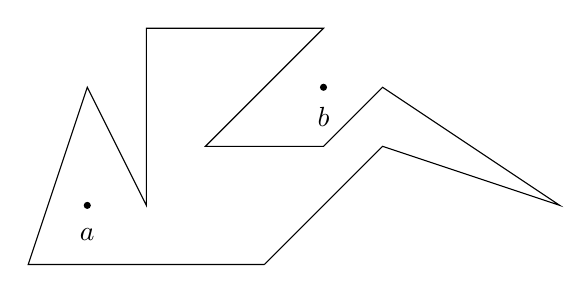
\begin{tikzpicture}[scale=0.75]
%\draw (0,0)--(2,-2)--(3,1)--(5,1)--(2,3)--(1,2)--(-1,2)--(1,4)--(-2,4)--(-2,1)--(-3,3)--(-4,0)--(0,0);
\draw (0,0)--(2,2)--(5,1)--(2,3)--(1,2)--(-1,2)--(1,4)--(-2,4)--(-2,1)--(-3,3)--(-4,0)--(0,0);

\draw[fill] (-3,1) circle [radius=0.05];
\node at (-3,0.5) {$a$};
\draw[fill] (1,3) circle [radius=0.05];
\node at (1,2.5) {$b$};
\end{tikzpicture}
\end{center}

一种方便的解法是从该点向任意方向发出一条\emph{射线}，并计算它与多边形边界相交的次数。若次数为奇数，点在多边形内部；若为偶数，点在多边形外部。

\begin{samepage}
例如，可以发出如下射线：
\begin{center}
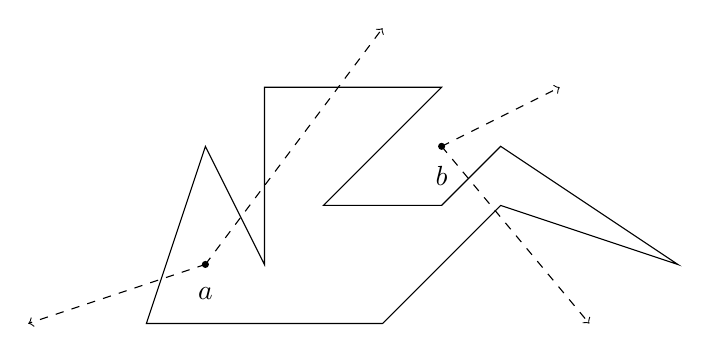
\begin{tikzpicture}[scale=0.75]
\draw (0,0)--(2,2)--(5,1)--(2,3)--(1,2)--(-1,2)--(1,4)--(-2,4)--(-2,1)--(-3,3)--(-4,0)--(0,0);

\draw[fill] (-3,1) circle [radius=0.05];
\node at (-3,0.5) {$a$};
\draw[fill] (1,3) circle [radius=0.05];
\node at (1,2.5) {$b$};

\draw[dashed,->] (-3,1)--(-6,0);
\draw[dashed,->] (-3,1)--(0,5);

\draw[dashed,->] (1,3)--(3.5,0);
\draw[dashed,->] (1,3)--(3,4);
\end{tikzpicture}
\end{center}
\end{samepage}

从 $a$ 发出的两条射线分别与多边形边界相交 1 次和 3 次，所以 $a$ 在多边形内部。相应地，从 $b$ 发出的两条射线分别相交 0 次和 2 次，所以 $b$ 在多边形外部。

\section{多边形面积}

计算多边形面积的通用公式有时称为\key{鞋带公式}：\index{shoelace formula}
\[\frac{1}{2} |\sum_{i=1}^{n-1} (p_i \times p_{i+1})| =
\frac{1}{2} |\sum_{i=1}^{n-1} (x_i y_{i+1} - x_{i+1} y_i)|, \]
其中顶点按多边形边界上的相邻顺序排列为 $p_1=(x_1,y_1)$、$p_2=(x_2,y_2)$、$\ldots$、$p_n=(x_n,y_n)$，并且首尾顶点相同，即 $p_1=p_n$。

例如，下列多边形的面积
\begin{center}
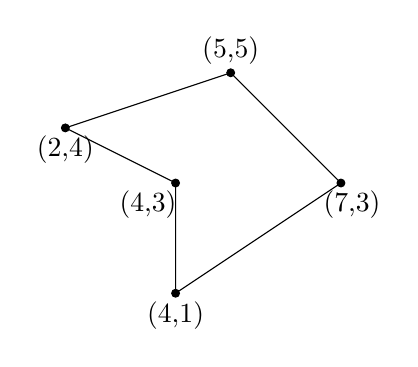
\begin{tikzpicture}[scale=0.7]
\filldraw (4,1.4) circle (2pt);
\filldraw (7,3.4) circle (2pt);
\filldraw (5,5.4) circle (2pt);
\filldraw (2,4.4) circle (2pt);
\filldraw (4,3.4) circle (2pt);
\node (1) at (4,1) {(4,1)};
\node (2) at (7.2,3) {(7,3)};
\node (3) at (5,5.8) {(5,5)};
\node (4) at (2,4) {(2,4)};
\node (5) at (3.5,3) {(4,3)};
\path[draw] (4,1.4) -- (7,3.4) -- (5,5.4) -- (2,4.4) -- (4,3.4) -- (4,1.4);
\end{tikzpicture}
\end{center}
为
\[\frac{|(2\cdot5-5\cdot4)+(5\cdot3-7\cdot5)+(7\cdot1-4\cdot3)+(4\cdot3-4\cdot1)+(4\cdot4-2\cdot3)|}{2} = 17/2.\]

该公式的思想是遍历若干梯形，其中一条边是多边形的一条边，另一条边位于水平直线 $y=0$ 上。例如：
\begin{center}
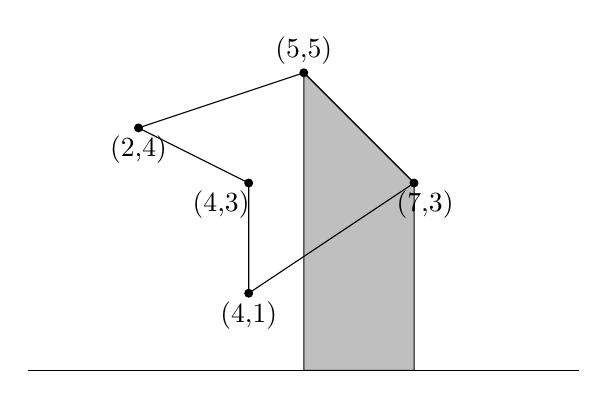
\begin{tikzpicture}[scale=0.7]
\path[draw,fill=lightgray] (5,5.4) -- (7,3.4) -- (7,0) -- (5,0) -- (5,5.4);
\filldraw (4,1.4) circle (2pt);
\filldraw (7,3.4) circle (2pt);
\filldraw (5,5.4) circle (2pt);
\filldraw (2,4.4) circle (2pt);
\filldraw (4,3.4) circle (2pt);
\node (1) at (4,1) {(4,1)};
\node (2) at (7.2,3) {(7,3)};
\node (3) at (5,5.8) {(5,5)};
\node (4) at (2,4) {(2,4)};
\node (5) at (3.5,3) {(4,3)};
\path[draw] (4,1.4) -- (7,3.4) -- (5,5.4) -- (2,4.4) -- (4,3.4) -- (4,1.4);
\draw (0,0) -- (10,0);
\end{tikzpicture}
\end{center}
这种梯形的面积为
\[(x_{i+1}-x_{i}) \frac{y_i+y_{i+1}}{2},\]
其中多边形的两个顶点为 $p_i$ 与 $p_{i+1}$。若 $x_{i+1}>x_i$，面积取正；若 $x_{i+1}<x_i$，面积取负。

多边形面积是所有此类梯形面积之和，由此得到公式
\[|\sum_{i=1}^{n-1} (x_{i+1}-x_{i}) \frac{y_i+y_{i+1}}{2}| =
\frac{1}{2} |\sum_{i=1}^{n-1} (x_i y_{i+1} - x_{i+1} y_i)|.\]

注意，需要对总和取绝对值，因为沿多边形边界按顺时针或逆时针方向遍历时，总和可能分别为正或为负。

\subsubsection{Pick 定理}

\index{Pick's theorem}

若多边形所有顶点的坐标均为整数，\key{Pick 定理}提供了另一种计算面积的方法。根据 Pick 定理，多边形面积为
\[ a + b/2 -1,\]
其中 $a$ 是多边形内部的整点数，$b$ 是边界上的整点数。

例如，下列多边形的面积
\begin{center}
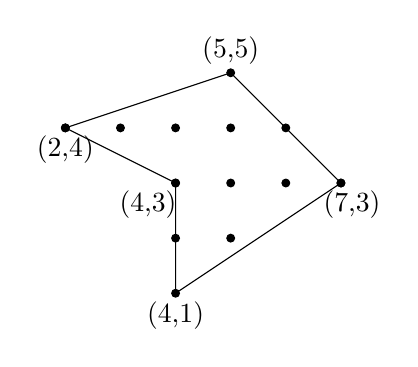
\begin{tikzpicture}[scale=0.7]
\filldraw (4,1.4) circle (2pt);
\filldraw (7,3.4) circle (2pt);
\filldraw (5,5.4) circle (2pt);
\filldraw (2,4.4) circle (2pt);
\filldraw (4,3.4) circle (2pt);
\node (1) at (4,1) {(4,1)};
\node (2) at (7.2,3) {(7,3)};
\node (3) at (5,5.8) {(5,5)};
\node (4) at (2,4) {(2,4)};
\node (5) at (3.5,3) {(4,3)};
\path[draw] (4,1.4) -- (7,3.4) -- (5,5.4) -- (2,4.4) -- (4,3.4) -- (4,1.4);

\filldraw (2,4.4) circle (2pt);
\filldraw (3,4.4) circle (2pt);
\filldraw (4,4.4) circle (2pt);
\filldraw (5,4.4) circle (2pt);
\filldraw (6,4.4) circle (2pt);

\filldraw (4,3.4) circle (2pt);
\filldraw (5,3.4) circle (2pt);
\filldraw (6,3.4) circle (2pt);
\filldraw (7,3.4) circle (2pt);

\filldraw (4,2.4) circle (2pt);
\filldraw (5,2.4) circle (2pt);
\end{tikzpicture}
\end{center}
为 $6+7/2-1=17/2$。

\section{距离函数}

\index{distance function}
\index{Euclidean distance}
\index{Manhattan distance}

\key{距离函数}定义两点之间的距离。常用的距离函数是\key{欧几里得距离}，点 $(x_1,y_1)$ 与 $(x_2,y_2)$ 之间的距离为
\[\sqrt{(x_2-x_1)^2+(y_2-y_1)^2}.\]
另一种距离函数是\key{曼哈顿距离}，点 $(x_1,y_1)$ 与 $(x_2,y_2)$ 之间的距离为
\[|x_1-x_2|+|y_1-y_2|.\]
\begin{samepage}
例如，考虑下图：
\begin{center}
\begin{tikzpicture}

\draw[fill] (2,1) circle [radius=0.05];
\draw[fill] (5,2) circle [radius=0.05];

\node at (2,0.5) {$(2,1)$};
\node at (5,1.5) {$(5,2)$};

\draw[dashed] (2,1) -- (5,2);

\draw[fill] (5+2,1) circle [radius=0.05];
\draw[fill] (5+5,2) circle [radius=0.05];

\node at (5+2,0.5) {$(2,1)$};
\node at (5+5,1.5) {$(5,2)$};

\draw[dashed] (5+2,1) -- (5+2,2);
\draw[dashed] (5+2,2) -- (5+5,2);

\node at (3.5,-0.5) {欧几里得距离};
\node at (5+3.5,-0.5) {曼哈顿距离};
\end{tikzpicture}
\end{center}
\end{samepage}
两点间的欧几里得距离为
\[\sqrt{(5-2)^2+(2-1)^2}=\sqrt{10}\]
曼哈顿距离为
\[|5-2|+|2-1|=4.\]
下图分别展示在欧几里得距离与曼哈顿距离下，到中心点距离不超过 1 的区域：
\begin{center}
\begin{tikzpicture}

\draw[fill=gray!20] (0,0) circle [radius=1];
\draw[fill] (0,0) circle [radius=0.05];

\node at (0,-1.5) {欧几里得距离};

\draw[fill=gray!20] (5+0,1) -- (5-1,0) -- (5+0,-1) -- (5+1,0) -- (5+0,1);
\draw[fill] (5,0) circle [radius=0.05];
\node at (5,-1.5) {曼哈顿距离};
\end{tikzpicture}
\end{center}

\subsubsection{旋转坐标系}

有些问题用曼哈顿距离代替欧几里得距离后更容易解决。例如，给定二维平面上的 $n$ 个点，要求计算任意两点之间的最大曼哈顿距离。

考虑下面这组点：
\begin{center}
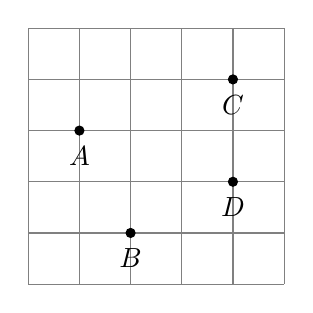
\begin{tikzpicture}[scale=0.65]
\draw[color=gray] (-1,-1) grid (4,4);

\filldraw (0,2) circle (2.5pt);
\filldraw (3,3) circle (2.5pt);
\filldraw (1,0) circle (2.5pt);
\filldraw (3,1) circle (2.5pt);

\node at (0,1.5) {$A$};
\node at (3,2.5) {$C$};
\node at (1,-0.5) {$B$};
\node at (3,0.5) {$D$};
\end{tikzpicture}
\end{center}
点 $B$ 与 $C$ 之间的曼哈顿距离最大，为 5：
\begin{center}
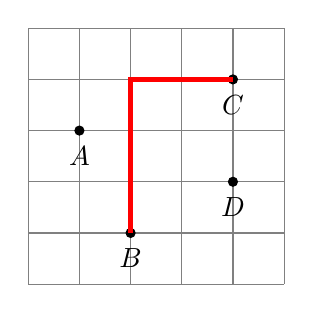
\begin{tikzpicture}[scale=0.65]
\draw[color=gray] (-1,-1) grid (4,4);

\filldraw (0,2) circle (2.5pt);
\filldraw (3,3) circle (2.5pt);
\filldraw (1,0) circle (2.5pt);
\filldraw (3,1) circle (2.5pt);

\node at (0,1.5) {$A$};
\node at (3,2.5) {$C$};
\node at (1,-0.5) {$B$};
\node at (3,0.5) {$D$};

\path[draw=red,thick,line width=2pt] (1,0) -- (1,3) -- (3,3);
\end{tikzpicture}
\end{center}

处理曼哈顿距离时，一种实用技巧是把整个坐标系旋转 45 度，使点 $(x,y)$ 变为 $(x+y,y-x)$。例如，旋转上述各点后得到：

\begin{center}
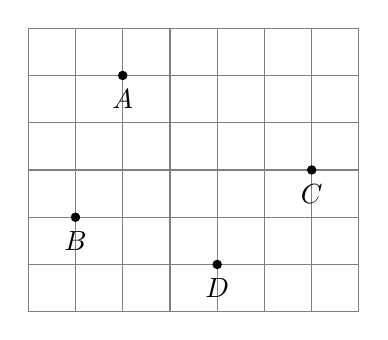
\begin{tikzpicture}[scale=0.6]
\draw[color=gray] (0,-3) grid (7,3);

\filldraw (2,2) circle (2.5pt);
\filldraw (6,0) circle (2.5pt);
\filldraw (1,-1) circle (2.5pt);
\filldraw (4,-2) circle (2.5pt);

\node at (2,1.5) {$A$};
\node at (6,-0.5) {$C$};
\node at (1,-1.5) {$B$};
\node at (4,-2.5) {$D$};
\end{tikzpicture}
\end{center}
最大距离如下所示：
\begin{center}
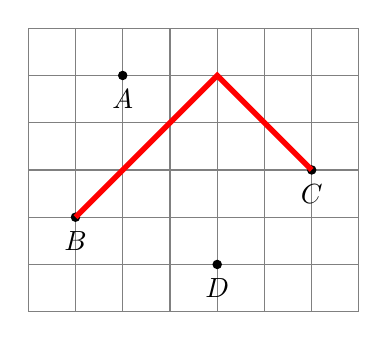
\begin{tikzpicture}[scale=0.6]
\draw[color=gray] (0,-3) grid (7,3);

\filldraw (2,2) circle (2.5pt);
\filldraw (6,0) circle (2.5pt);
\filldraw (1,-1) circle (2.5pt);
\filldraw (4,-2) circle (2.5pt);

\node at (2,1.5) {$A$};
\node at (6,-0.5) {$C$};
\node at (1,-1.5) {$B$};
\node at (4,-2.5) {$D$};

\path[draw=red,thick,line width=2pt] (1,-1) -- (4,2) -- (6,0);
\end{tikzpicture}
\end{center}

考虑两点 $p_1=(x_1,y_1)$ 和 $p_2=(x_2,y_2)$，旋转后的坐标分别为 $p'_1=(x'_1,y'_1)$ 和 $p'_2=(x'_2,y'_2)$。此时，$p_1$ 与 $p_2$ 之间的曼哈顿距离有两种等价表示：
\[|x_1-x_2|+|y_1-y_2| = \max(|x'_1-x'_2|,|y'_1-y'_2|)\]

例如，若 $p_1=(1,0)$、$p_2=(3,3)$，旋转后坐标为 $p'_1=(1,-1)$、$p'_2=(6,0)$，曼哈顿距离为
\[|1-3|+|0-3| = \max(|1-6|,|-1-0|) = 5.\]

旋转坐标后可以分别考虑 x、y 坐标，从而简化曼哈顿距离的处理。要最大化两点之间的曼哈顿距离，应找到旋转后坐标使下式最大的两个点：
\[\max(|x'_1-x'_2|,|y'_1-y'_2|).\]
这很容易做到，因为旋转后坐标的水平差或垂直差中必有一个达到最大值。
